\documentclass[french, 11pt]{assets/biso}

\newcommand{\reportyear}{2024}
\newcommand{\halcollectionid}{UNIV-PARIS-SACLAY}
\newcommand{\labacronym}{UPSaclay}
\newcommand{\labfullname}{Université Paris-Saclay}
\newcommand{\datafetchdate}{24/09/2025}
\newcommand{\watermarktext}{}

\newcommand{\anrprojectsinfo}{Le nombre d'entités affichées a été limité à 20. Dans l'API, 1637 entités ont été trouvées.\\}
\newcommand{\chaptersinfo}{}
\newcommand{\collaborationsnb}{2957}
\newcommand{\institutionsnb}{1269}
\newcommand{\countriesnb}{82}
\newcommand{\collaborationmapworldinfo}{\emoji{warning} Le traitement des données a été limité par le nombre maximal d'entités téléchargeables (1000). Des données peuvent être manquantes ou les valeurs peuvent être inférieures aux valeurs réelles. \\}
\newcommand{\collaborationmapeuropeinfo}{\emoji{warning} Le traitement des données a été limité par le nombre maximal d'entités téléchargeables (1000). Des données peuvent être manquantes ou les valeurs peuvent être inférieures aux valeurs réelles. \\}
\newcommand{\collaborationnamesinfo}{Le nombre d'entités affichées a été limité à 40. Dans l'API, 14322 entités ont été trouvées.\\}
\newcommand{\conferencesinfo}{Le nombre d'entités affichées a été limité à 40. Dans l'API, 2609 entités ont été trouvées.\\}
\newcommand{\europeanprojectsinfo}{Le nombre d'entités affichées a été limité à 20. Dans l'API, 551 entités ont été trouvées.\\}
\newcommand{\bsojournalsnbworks}{1000}
\newcommand{\bsojournalsnbworksfoundinbso}{792}
\newcommand{\bsojournalsnbjournals}{503}
\newcommand{\bsojournalsbsoversion}{2024Q4}
\newcommand{\journalsinfo}{\emoji{warning} Le traitement des données a été limité par le nombre maximal d'entités téléchargeables (1000). Des données peuvent être manquantes ou les valeurs peuvent être inférieures aux valeurs réelles. \\}
\newcommand{\journalshalinfo}{Le nombre d'entités affichées a été limité à 40. Dans l'API, 3407 entités ont été trouvées.\\}
\newcommand{\oaworksperiod}{2020 - 2024}
\newcommand{\openaccessworksinfo}{}
\newcommand{\privatesectorcollaborationsinfo}{\emoji{warning} Le traitement des données a été limité par le nombre maximal d'entités téléchargeables (1000). Des données peuvent être manquantes ou les valeurs peuvent être inférieures aux valeurs réelles. \\}
\newcommand{\workstypeinfo}{}



\title{Bilan \\ Science \\ Ouverte}

\author{Direction des bibliothèques, de l’information et de la science ouverte}

\date{Année \reportyear}

\subtitle{\textbf{Laboratoire \labacronym} \\
  \medskip
  \labfullname
}


\reporter{Reporter Name}
\reporteremail{reporter.email@example.com}



\begin{document}

\renewcommand{\arraystretch}{1.5}

%%%%% WATERMARK %%%%%

% https://tex.stackexchange.com/questions/118939/add-watermark-that-overlays-the-images
\AddToHook{shipout/foreground}{
 \begin{tikzpicture}[overlay, remember picture]
   \node[rotate=45, scale=8] at (current page) {\addfontfeature{Color=gray,Opacity=0.1}BROUILLON};
  \end{tikzpicture}    
}

%%%%% END WATERMARK %%%%%



\maketitle

\tableofcontents

\pagebreak



\section{Introduction}

Ce BiSO (Bilan Science Ouverte) a pour objectif de suivre l'évolution des indicateurs clés liés aux productions scientifiques de votre unité. Ce document, principalement fondé sur les données de HAL, vous permettra de monitorer les actions de diffusion en vue de l'évaluation HCERES.

L'analyse se concentre sur plusieurs éléments essentiels, tels que la productivité scientifique, la visibilité des publications et les collaborations internationales. En étudiant ces indicateurs, nous souhaitons mettre en
lumière les atouts et les opportunités de l'unité tout en identifiant les secteurs nécessitant des améliorations.

Ce bilan a également pour but de contextualiser les évolutions par rapport aux objectifs stratégiques de l'unité. Les données collectées seront analysées afin de formuler des recommandations pratiques visant à renforcer l'impact
scientifique et académique de l'unité.

Ce rapport sera élaboré chaque année et diffusé en interne au sein de votre laboratoire, dans le but de préparer au mieux la prochaine évaluation HCERES.



\pagebreak

\section{Liste des revues}

{
  \footnotesize
  \begin{longtable}{p{.55\linewidth}P{.08\linewidth}P{.11\linewidth}P{.11\linewidth}}
\caption{Liste des revues}
\label{tab_journals}\\
\toprule
Revue & Nombre de publications & Status des accès ouverts des publications & APC payés \\
\midrule
Volume 3A: Combustion, Fuels, and Emissions & \makecell{3} & \makecell{2 closed, \\ 1 green} & \makecell{} \\
Proceedings of the Combustion Institute & \makecell{7} & \makecell{6 other, \\ 1 hybrid} & \makecell{2 980 USD} \\
International Journal of Heat and Mass Transfer & \makecell{1} & \makecell{1 other} & \makecell{} \\
Chemical Engineering Research and Design & \makecell{2} & \makecell{2 green} & \makecell{} \\
Combustion and Flame & \makecell{4} & \makecell{4 other} & \makecell{} \\
Volume 3B: Combustion, Fuels, and Emissions & \makecell{1} & \makecell{1 green} & \makecell{} \\
Plasma Sources Science and Technology & \makecell{4} & \makecell{2 closed, \\ 2 green} & \makecell{} \\
Journal of Engineering for Gas Turbines and Power & \makecell{3} & \makecell{2 closed, \\ 1 green} & \makecell{} \\
Aerospace & \makecell{1} & \makecell{1 gold} & \makecell{1 600 CHF} \\
Applications in Energy and Combustion Science & \makecell{4} & \makecell{4 gold} & \makecell{2 000 USD, \\ 2 000 USD, \\ 2 000 USD, \\ 2 000 USD} \\
AIAA Journal & \makecell{1} & \makecell{1 green} & \makecell{} \\
Applied Physics B & \makecell{3} & \makecell{3 green} & \makecell{} \\
AIAA SCITECH 2023 Forum & \makecell{1} & \makecell{1 green} & \makecell{} \\
Computers \& Fluids & \makecell{1} & \makecell{1 green} & \makecell{} \\
International Journal of Multiphase Flow & \makecell{1} & \makecell{1 closed} & \makecell{} \\
CEAS Space Journal & \makecell{1} & \makecell{1 green} & \makecell{} \\
Frontiers in Physics & \makecell{1} & \makecell{1 gold} & \makecell{2 490 USD} \\
Biophysical Journal & \makecell{1} & \makecell{1 hybrid} & \makecell{2 500 USD} \\
Journal of Thermophysics and Heat Transfer & \makecell{1} & \makecell{1 green} & \makecell{} \\
Journal of Aerosol Science & \makecell{1} & \makecell{1 green} & \makecell{} \\
International Journal of Thermal Sciences & \makecell{1} & \makecell{1 green} & \makecell{} \\
Proceeding of International Heat Transfer Conference 17 & \makecell{1} & \makecell{1 green} & \makecell{} \\
\bottomrule
\end{longtable}

}

\pagebreak

\section{Liste des conférences}

\begin{figure}[!h]
  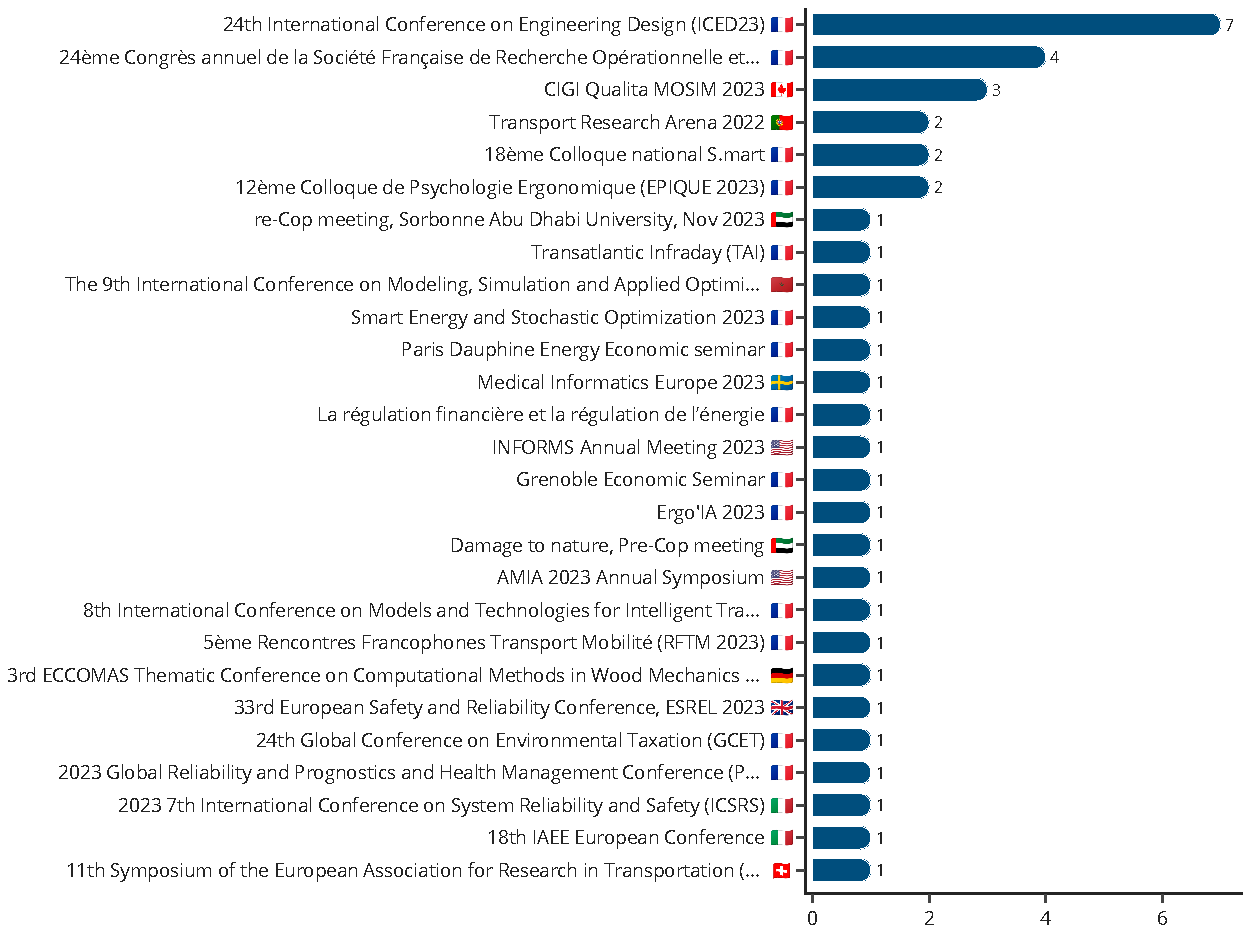
\includegraphics[width=\textwidth]{figures/conferences.pdf}
  \centering
  \caption{Conférences}
  \label{fig_conferences}
\end{figure}


\pagebreak

\section{Liste des chapitres}

{
  \footnotesize
  \begin{longtable}{p{.4\linewidth}p{.35\linewidth}p{.15\linewidth}}
\caption{Liste des chapitres}
\label{tab_chapters}\\
\toprule
Titre du chapitre & Titre du livre & Éditeur \\
\midrule
Concurrence et régulation & Commentaire J. Mégret : L’énergie &  \\
La place du charbon dans l’Union européenne & Commerce transnational et industries extractives : entre singularité et pérennité d’un modèle &  \\
Démocratie environnementale : quelle(s) réalité(s) derrière les mots ? & Le droit économique de l’environnement : Acteurs et méthodes & Mare \& Martin \\
Ethique, science et gouvernance internationale en temps de pandémie & Sciences et pandémies : quelle éthique pour demain ? & éditions Erès \\
A la recherche de l’esprit de solidarité énergétique & Union européenne et solidarité(s) & Bruylant \\
Une certaine idée du service public culturel. Du 19ème au début du 20ème siècle & L’artiste, l’administrateur et le juge. L’invention du service public culturel. Le rôle du Conseil d’Etat, Actes du colloque des 26 et 27 novembre 2021, organisé par le Comité d’histoire du Conseil d’Etat et de la juridiction administrative et le Comité d’histoire du ministère de la culture & La rumeur libre éditions \\
Le Parlement comme contre-pouvoir sous la Ve République. Les enseignements des élections législatives de juin 2022 & Institutions et contre-pouvoir. Représentation, contrôle et ordre constitutionnel au prisme du droit constitutionnel comparé & Nihon Hyoron Sha \\
Le serment du chef de l’État & Le Serment. Perspectives juridiques contemporaines & Société de législations comparée \\
La 9e question mise au programme du Congrès international de droit comparé de 1900 & Mélanges en l’honneur du Professeur Ken Hasegawa & Mare \& Martin \\
Le permis de construire sur le domaine public : entre protection du domaine et simplification des autorisations d’urbanisme. À propos de l’article R. 431-13 du code de l’urbanisme & Droit de l’Aménagement de l’Urbanisme de l’Habitat, 27e éd. & Le Moniteur \\
Essais nucléaires et statut colonial de la Polynésie française : la rhétorique indépendantiste au sein de l’Organisation des Nations Unies & Le traitement juridique contemporain du fait nucléaire français en Polynésie française & Pedone \\
La réponse de l’Union européenne à la crise énergétique : unie dans le conflit ? & La conflictualité dans l’Union européenne : menace existentielle ou catalyseur d’intégration ? & Bruylant \\
A propos des accords bilatéraux de coopération récemment conclus avec trois Etats voisins (traités d’Aix-la-Chapelle, du Quirinal et de Barcelone) & Annuaire français de droit international (AFDI) &  \\
La typologie des régimes politiques à l’aune de la structure de l’exécutif & Les figures contemporaines du chef de l’État en régime parlementaire & Bruylant \\
La solidarité européenne à l’épreuve de la pandémie : bilan d’une stratégie vaccinale en clair-obscur & Ethique et gouvernance internationale de la recherche – Les enseignements de la pandémie de Covid-19 &  \\
L’utilisation du contrôle de proportionnalité par les juges européens en matière d’asile & Les juges européens face aux migrations & Anthémis \\
Préface & La déclaration Union européenne-Turquie, ambiguïtés et devenir d’un modèle de gestion des flux migratoires & Bruylant, collection Pratique(s) du droit international \\
\bottomrule
\end{longtable}

}


\pagebreak

\section{Typologie de la production scientifique}

\begin{figure}[!h]
  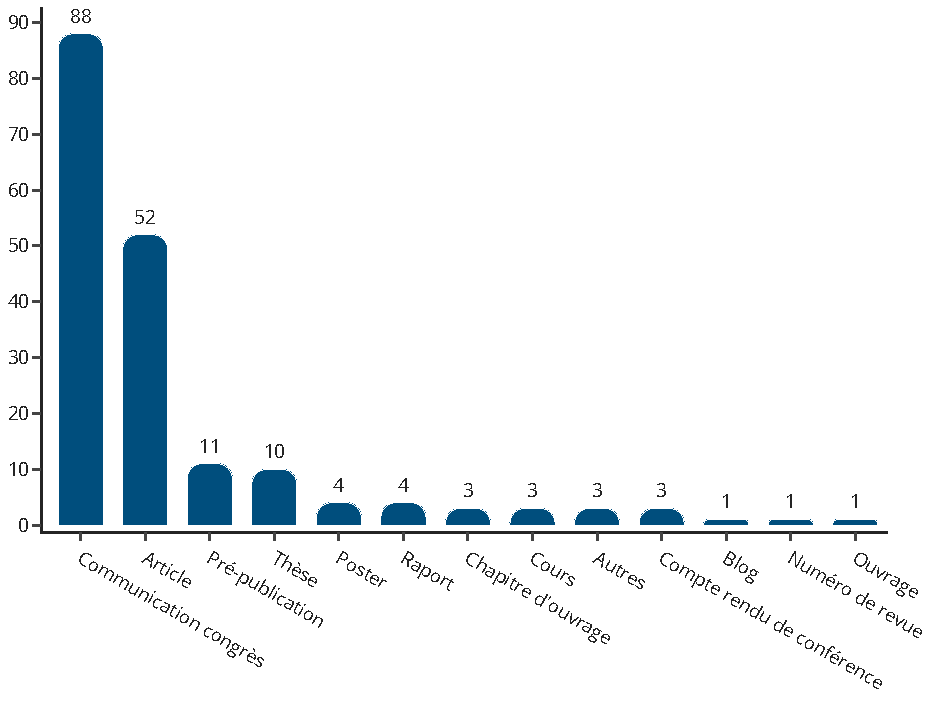
\includegraphics[width=\textwidth]{figures/document_types.pdf}
  \centering
  \caption{Types de documents}
  \label{fig_doc_type}
\end{figure}


\pagebreak

\section{Articles et Communication de congrès en accès libre} % Evolution sur une période de 5 ans (2020-2024)

\begin{figure}[!h]
  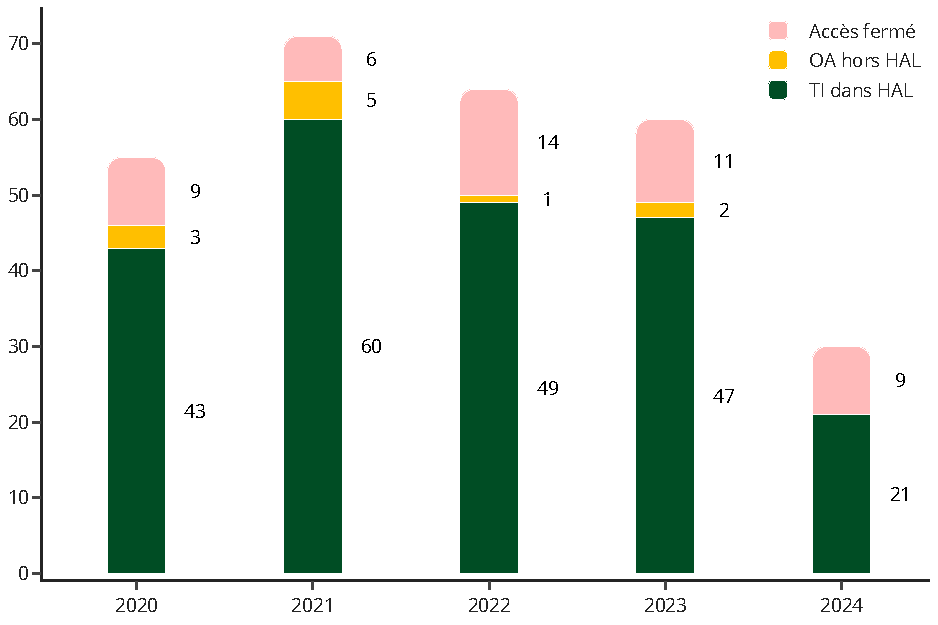
\includegraphics[width=\textwidth]{figures/open_access_works.pdf}
  \caption{Statut des accès ouverts des travaux sur la période \oaworksperiod}
  \label{fig_open_access_works}
\end{figure}


\pagebreak

\section{Carte des collaborations internationales}

{\collaborationsnb} collaborations parmi {\institutionsnb} institutions dans {\countriesnb} pays d'après la liste des articles avec un DOI dans HAL et les données de collaboration d'OpenAlex.

\begin{figure}[!h]
  \hspace{-.1\textwidth}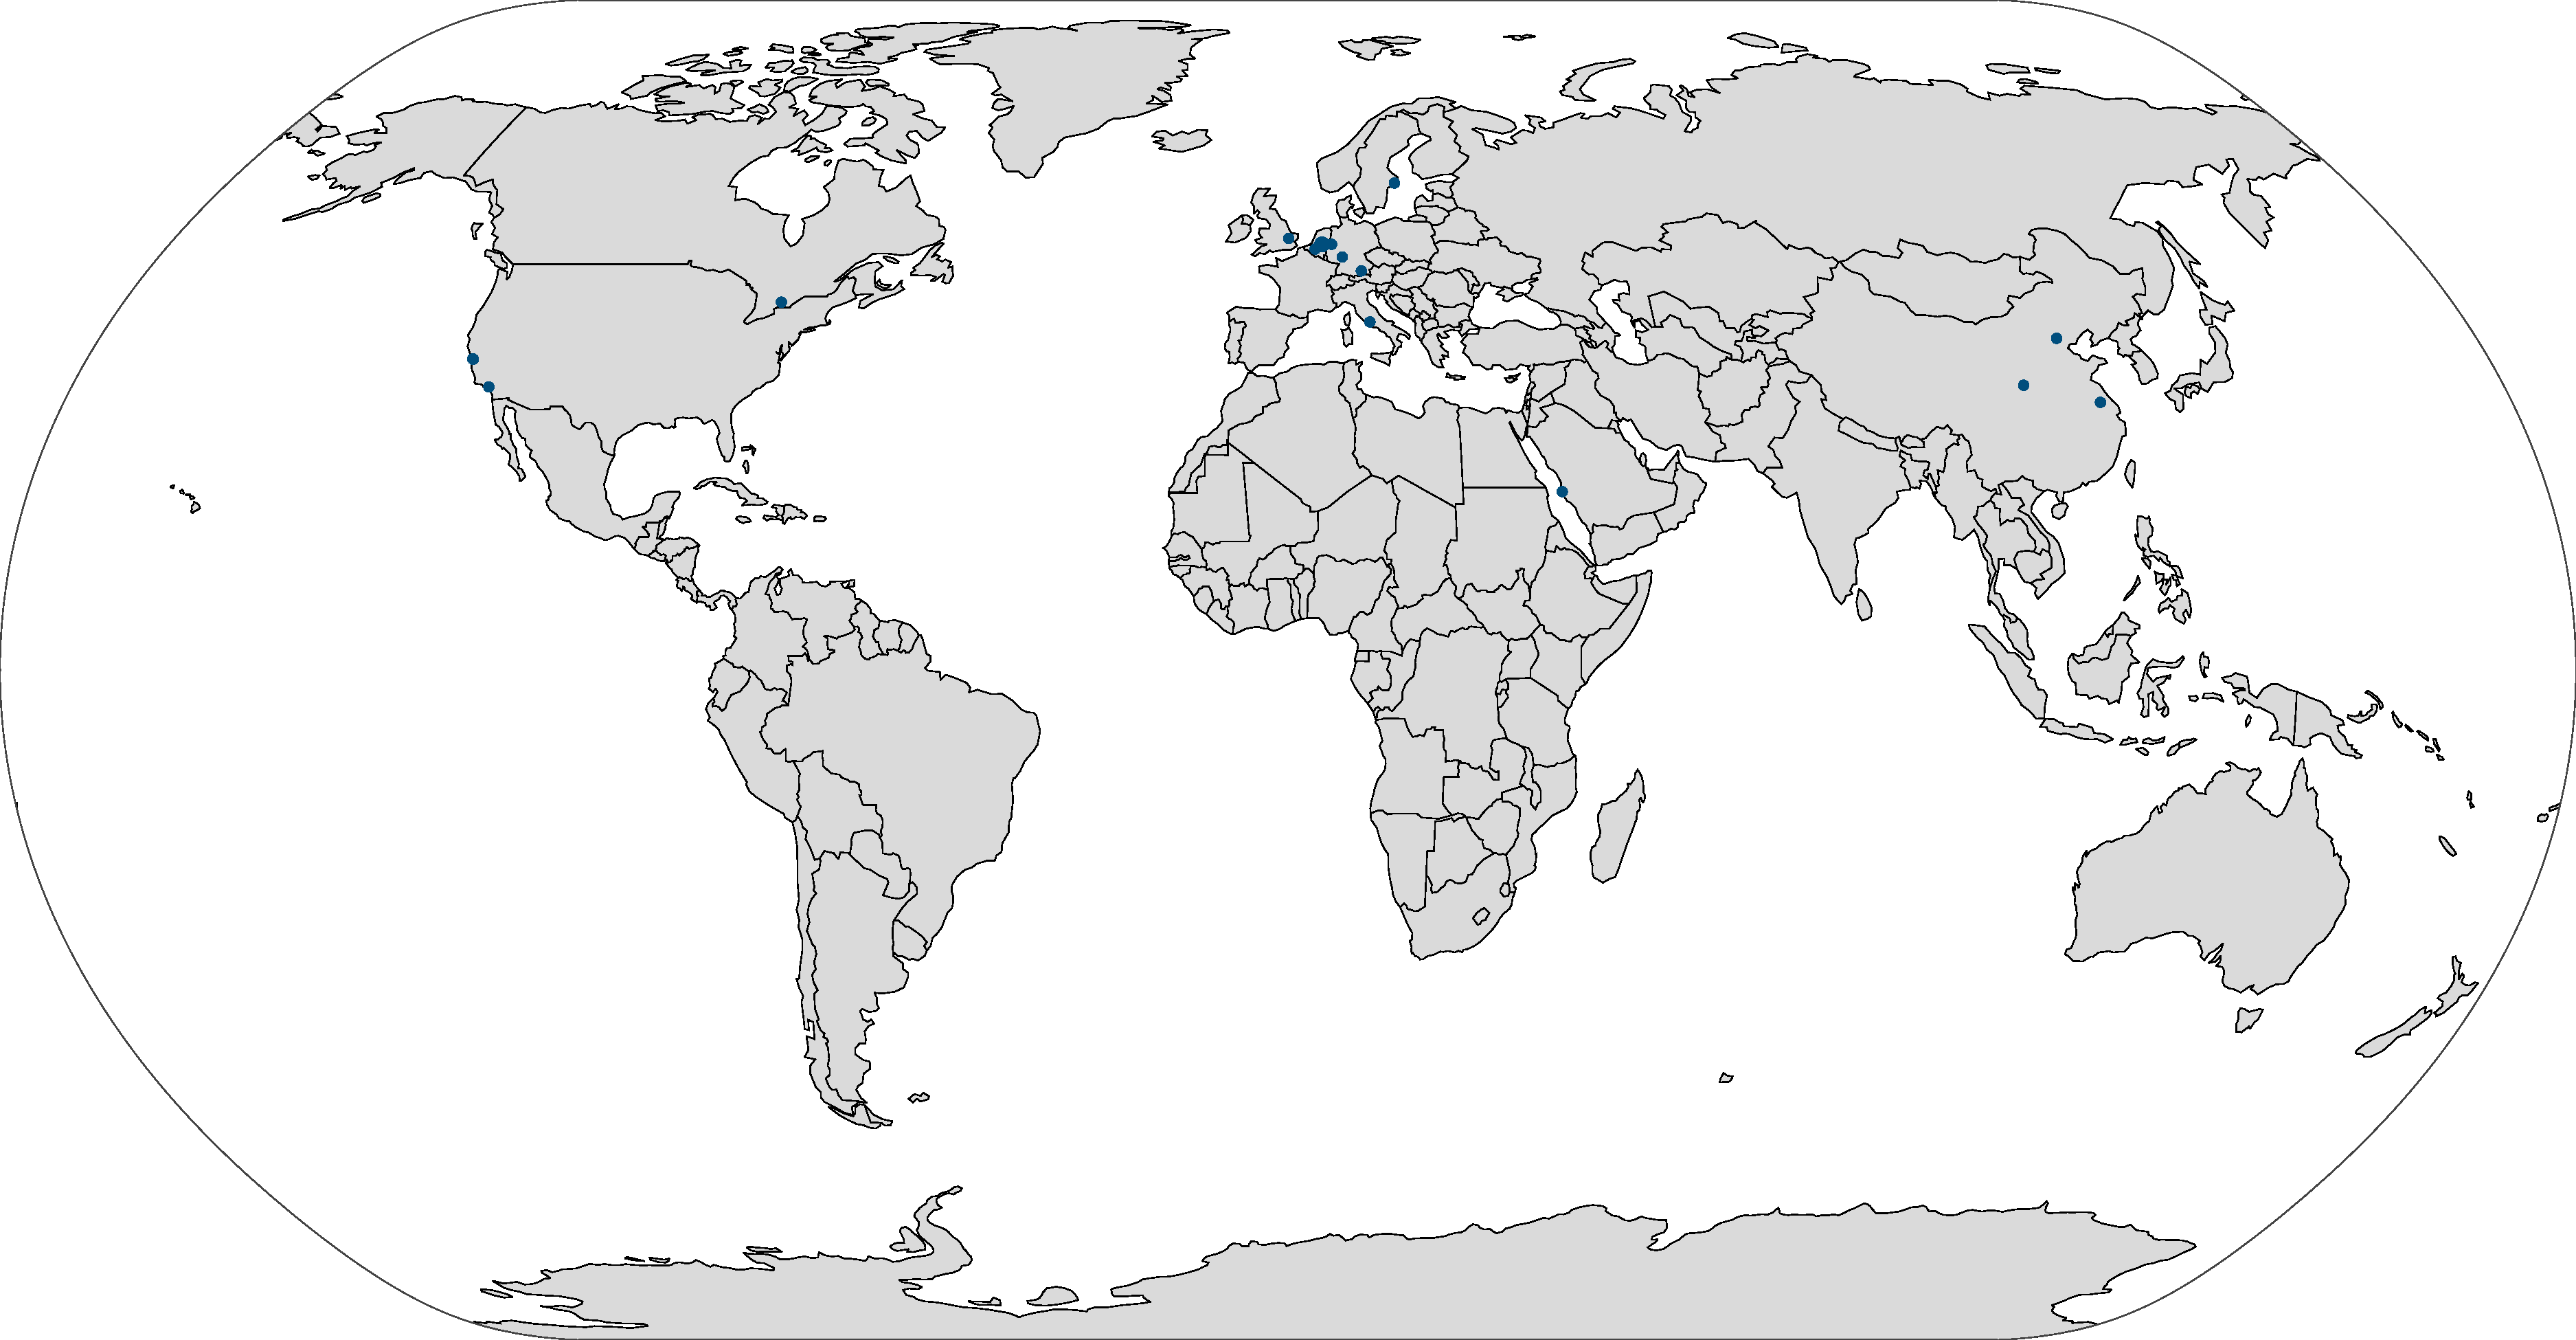
\includegraphics[width=1.2\textwidth]{figures/collaborations_map.pdf}
  \caption{Collaborations internationales hors France - Données : publications renseignées dans HAL avec un DOI en utilisant les métadonnées d'OpenAlex}
  \label{fig_collab_map}
\end{figure}

\pagebreak

\section{Carte des collaborations internationales - Focus sur l’Europe}

\begin{figure}[!h]
  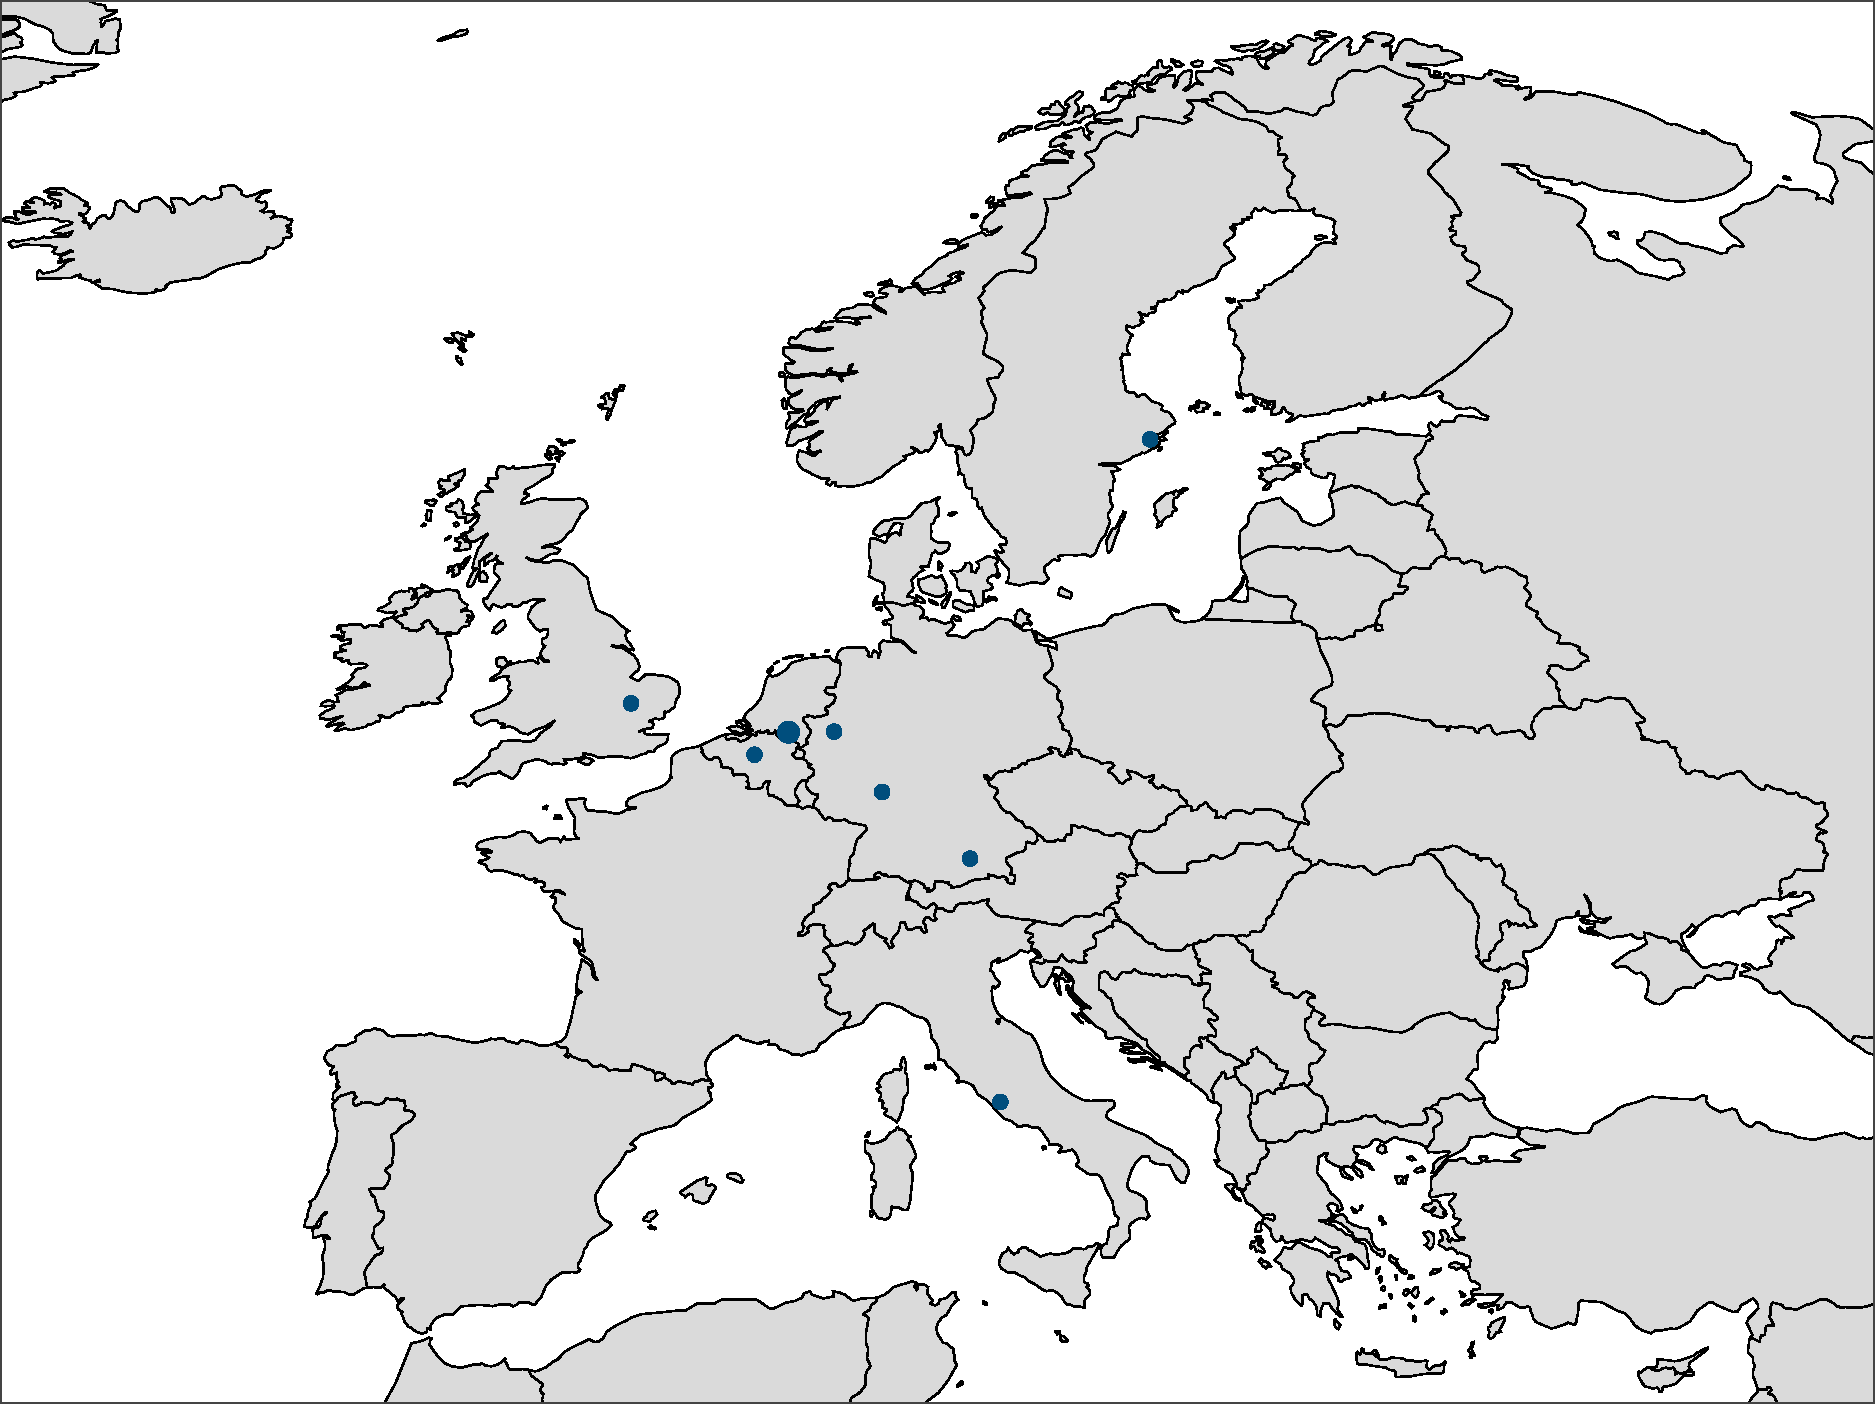
\includegraphics[width=\textwidth]{figures/collaborations_map_europe.pdf}
  \caption{Collaborations internationales hors France en 2024 - Zoom sur l'europe - Données : publications renseignées dans HAL avec un DOI en utilisant les métadonnées d'OpenAlex}
  \label{fig_collab_map_europe}
\end{figure}

\pagebreak

\section{Collaborations internationales par établissements}

\begin{figure}[!h]
  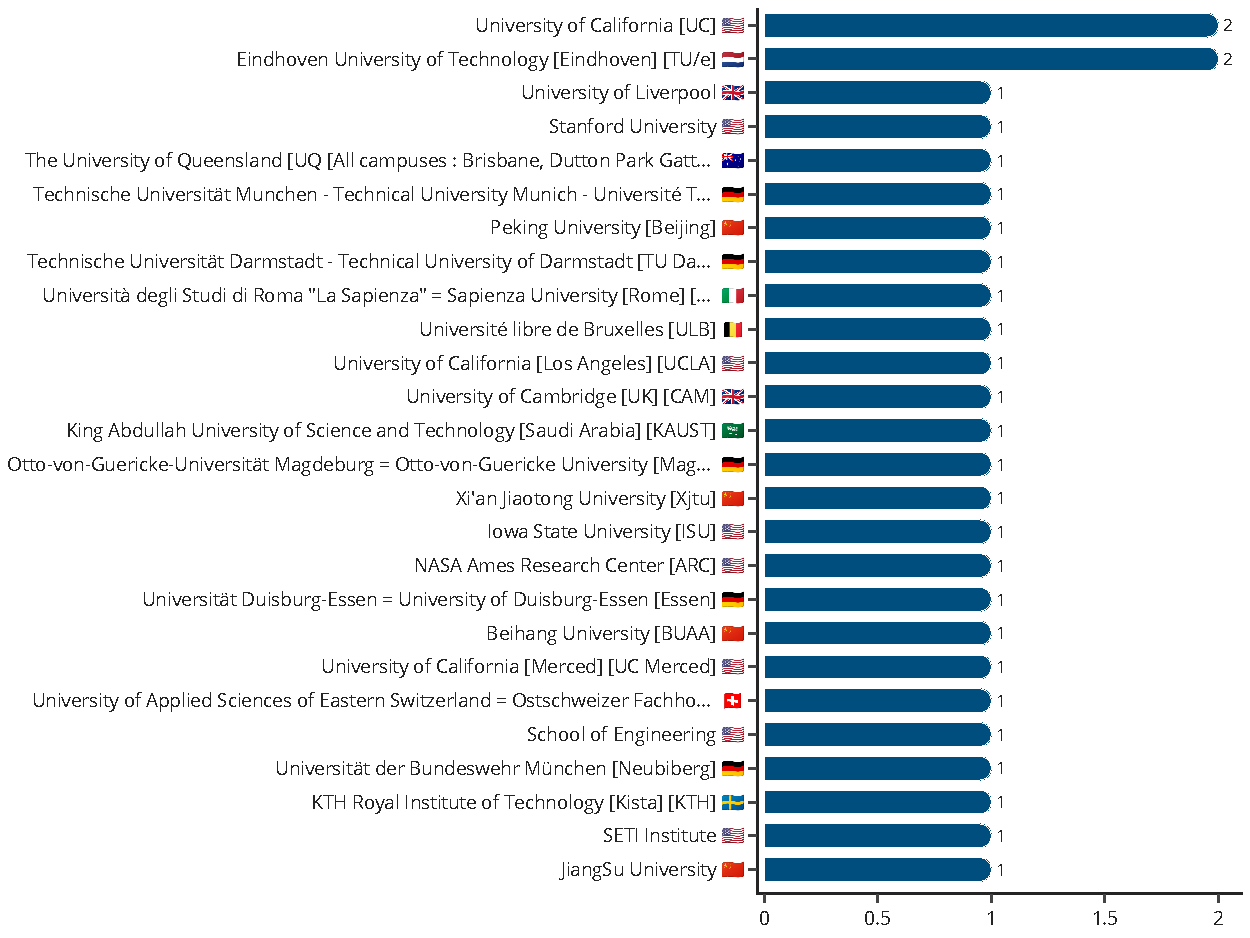
\includegraphics[width=\textwidth]{figures/international_collaborations.pdf}
  \caption{Collaborations internationales hors France en 2024 - Données : Nom des institutions renseignées dans HAL}
  \label{fig_collab_names}
\end{figure}

\pagebreak

\section{Collaborations (non académique) avec le secteur privé}


\pagebreak

\section{Publications liées à des projets européens}

\begin{figure}[!h]
  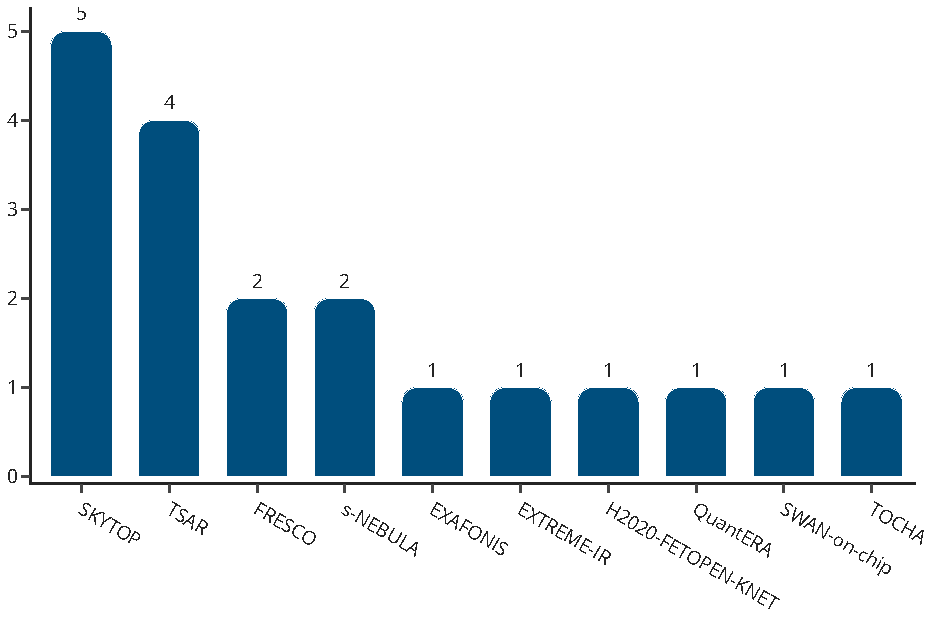
\includegraphics[width=.8\textwidth]{figures/eu_projects.pdf}
  \centering
  \caption{Projets Européens}
  \label{fig_eu_projects}
\end{figure}



\section{Publications liées à des projets ANR}

\begin{figure}[!h]
  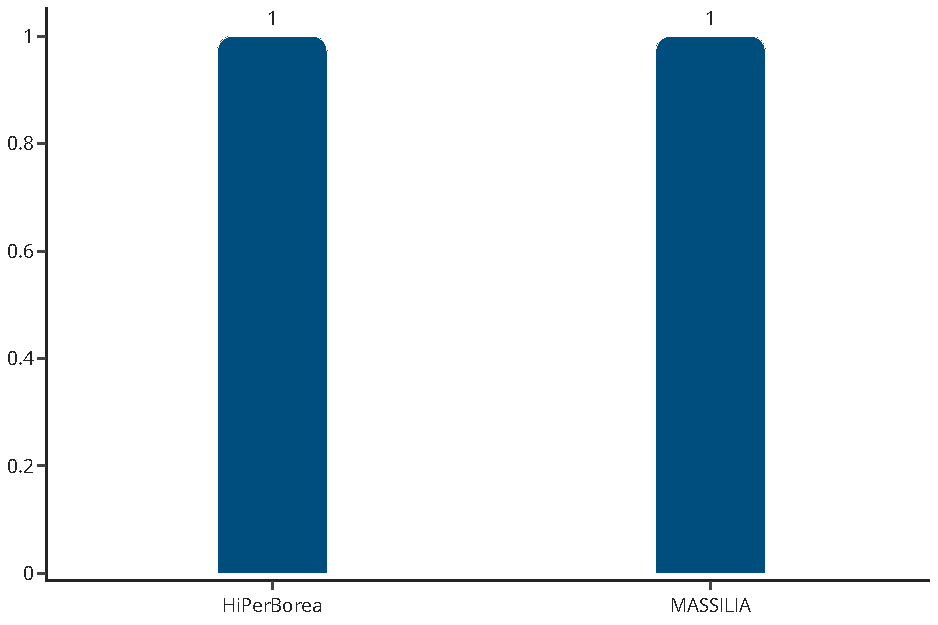
\includegraphics[width=.8\textwidth]{figures/anr_projects.pdf}
  \centering
  \caption{Projets ANR}
  \label{fig_anr_projects}
\end{figure}


\pagebreak

\section{Données - jeux de données partagés}



\section{Logiciels partagés}



\section{Cahiers de laboratoire partagés}




\pagebreak

\section{Les atouts du Laboratoire dans son engagement pour la science ouverte}

\begin{itemize}
  \item Publications dans des revues variées, favorisant la bibliodiversité.
  \item Très bonne prise en main de HAL par les chercheurs, pour un archivage et un Open access qui suit les prérogatives du CNRS. Les notices sont globalement bien renseignées avec des notices complètes et des affiliations complètes.
  \item Des projets ANR visibles et repérés dans HAL
  \item Formation et accompagnement des doctorants sur l’année (création 21 IdHAL)
  \item Une demi-journée dédiée aux données de la recherche en mars 2025 (échanges sur les données de la recherche dans des ateliers organisés par la DiBISO)
\end{itemize}


\section{Préconisations, pour aller plus loin}

\begin{itemize}
  \item Nouveauté : il est possible d’indiquer les jeux de données dans les liens HAL \say{champs ressource liée = on peut indiquer le DOI de jeux de données}
  \item Faire monter le taux de PDF, texte intégral disponible, pour faire avancer la lecture des publications.
\end{itemize}

\vfill

\paragraph{Rappel :} la loi pour la République Numérique permet aux auteurs travaillant dans une institution publique en France depuis 2016, de partager le postprint sur HAL, avec un embargo de 6 mois pour les disciplines STM et 1 an pour les SHS.

Des formations, des accompagnements peuvent être proposées par votre référent recherche pour guider les chercheurs. 




\makelastpagereport
 
\end{document}
